\documentclass[10pt]{article}
\usepackage[a4paper,margin=18mm,headsep=5mm]{geometry}
\usepackage{fontspec}
\usepackage{xeCJK}
\setmainfont{DejaVu Serif}
\setsansfont{DejaVu Sans}
\setmonofont{DejaVu Sans Mono}
\setCJKmainfont{Noto Serif CJK SC}
\setCJKsansfont{Noto Sans CJK SC}
\usepackage{amsmath,amssymb,mathtools,bm}
\usepackage{booktabs,tabularx,array,multirow}
\usepackage{graphicx}
\usepackage[dvipsnames,table]{xcolor}
\usepackage{hyperref}
\usepackage{enumitem}
\usepackage{fancyhdr}
\usepackage{caption}
\usepackage{microtype}

\definecolor{DeepBlue}{HTML}{145B8C}
\definecolor{SoftBlue}{HTML}{EAF3F8}
\definecolor{DeepOrange}{HTML}{B64A00}
\definecolor{SoftOrange}{HTML}{FFF2E8}
\definecolor{DeepGreen}{HTML}{087F5B}
\definecolor{SoftGray}{HTML}{F5F6F8}
\hypersetup{colorlinks=true,linkcolor=DeepBlue,urlcolor=DeepBlue,citecolor=DeepBlue}
\captionsetup{font=small,labelfont=bf}
\setlist{nosep,leftmargin=1.5em}
\setlength{\parindent}{1.5em}
\setlength{\parskip}{0.25em}
\pagestyle{fancy}
\fancyhf{}
\lhead{HT scale-head optimization note}
\rhead{2026-09-08}
\cfoot{\thepage}
\renewcommand{\headrulewidth}{0.3pt}

\newcommand{\E}{\mathbb{E}}
\newcommand{\R}{\mathbb{R}}
\newcommand{\sg}{\operatorname{sg}}
\newcommand{\softplus}{\operatorname{softplus}}
\newcommand{\Loss}{\mathcal{L}}
\newcommand{\norm}[1]{\left\lVert#1\right\rVert}

\title{\vspace{-1.5em}\textbf{小 $\nu$ 下异方差 Student-$t$ 的 scale-head 优化问题}\\[-0.1em]
\large 两个梯度失衡、两个候选修复及当前证据边界}
\author{Internal technical note for \emph{Much Ado About Noising}}
\date{2026-09-08}

\begin{document}
\maketitle
\vspace{-1.5em}

\noindent\fcolorbox{DeepBlue}{SoftBlue}{%
\begin{minipage}{0.965\linewidth}
\textbf{结论先行。}
数据上的联合 Student-$t$ 拟合偏好个位数 $\nu$，但端到端策略训练中，小 $\nu$ 会让共享特征收到的 scale-path 梯度相对 mean-path 快速衰减；现有 softplus scale 参数化还会对较大的绝对尺度施加额外链式衰减。这两个问题是\emph{不同的}：前者来自 Student-$t$ score 中的 $\nu/(\nu+q)$，后者来自 $\partial\log\sigma/\partial u$。候选方案 A 用 detached-mean Gaussian auxiliary 恢复 scale 梯度，并应配合直接预测 $s=\log\sigma$；候选方案 B 改用 scaled energy proper score，同样使用 log-scale 参数化。方案 B 对 mean gradient 有界，因而比 Gaussian 更抗长尾，但它不具有 Student-$t$ NLL 的 redescending influence，不能表述成“等价的 Student-$t$ 长尾抑制”。
\end{minipage}}

\section{问题设置与记号}

给定输入 $o$、动作块标签 $a\in\R^d$，网络共享特征为 $x=h_\theta(o)$，两个 head 分别预测位置 $\mu=\mu_\theta(x)$ 与标量尺度 $\sigma=\sigma_\theta(x)>0$。令
\begin{equation}
 r=\mu-a,\qquad S=\norm{r}^2,\qquad q=\frac{S}{\sigma^2},\qquad s=\log\sigma .
 \label{eq:notation}
\end{equation}
当前 GR00T action chunk 在 Bridge/Fractal 上有 $d=8\times7=56$ 个有效训练坐标；GR1 为 $d=8\times29=232$。以下统一使用\emph{每坐标平均}的 joint Student-$t$ negative log-likelihood（省略与 $\mu,\sigma$ 无关的常数）：
\begin{equation}
 \ell_T(\mu,s;\nu)
 =\frac{\nu+d}{2d}\log\!\left(1+\frac{q}{\nu}\right)+s .
 \label{eq:t-nll}
\end{equation}
对应的 heteroscedastic Gaussian（HG）loss 为
\begin{equation}
 \ell_G(\mu,s)=\frac{q}{2d}+s .
 \label{eq:hg-nll}
\end{equation}
这里的 $\nu$ 是整个 $d$ 维向量共享 radial scale 的 joint-$t$ 自由度，不是逐坐标自由度的求和。

\paragraph{为什么现在才暴露问题。}
冻结现有策略输出后重新做完整 joint likelihood calibration，得到的描述性最优值为 Fractal $\hat\nu=6.53$、Bridge $9.82$、RoboCasa-GR1 $5.66$；训练中表现较好的设置却分别使用了 $224,224,928$。这不意味着统计拟合错了，而是说明“固定预测上的 density fit”和“共享神经网络的端到端优化条件”不是同一个问题。

\section{问题一：小 $\nu$ 让 scale path 被 mean path 抢占}

\subsection{精确梯度恒等式}

对式~\eqref{eq:t-nll} 求导，记 $w=(\nu+d)/(\nu+q)$，得到
\begin{align}
 \nabla_\mu \ell_T
 &=\frac{w}{d\sigma^2}r,
 &
 \frac{\partial\ell_T}{\partial s}
 &=1-\frac{wq}{d}
 =\frac{\nu(d-q)}{d(\nu+q)}. 
 \label{eq:t-grads}
\end{align}
Gaussian loss 的对应梯度为
\begin{align}
 \nabla_\mu \ell_G&=\frac{r}{d\sigma^2},
 &
 \frac{\partial\ell_G}{\partial s}&=1-\frac{q}{d}.
 \label{eq:g-grads}
\end{align}
因此，在\emph{相同的特征、head、残差与尺度}上有两个精确关系：
\begin{equation}
 \nabla_\mu\ell_T=w\nabla_\mu\ell_G,
 \qquad
 \frac{\partial\ell_T}{\partial s}
 =\frac{\nu}{\nu+q}\frac{\partial\ell_G}{\partial s}.
 \label{eq:gradient-identities}
\end{equation}
进一步，把两个 head 对共享特征 $x$ 的 Jacobian 分别记作 $J_\mu,J_s$，则
\begin{equation}
 g_x^\mu=J_\mu^\top\nabla_\mu\ell_T,qquad
 g_x^\sigma=J_s^\top\frac{\partial\ell_T}{\partial s}.
\end{equation}
相对于 Gaussian，在每个样本上 scale/mean 的权重比额外乘上
\begin{equation}
 \frac{\nu/(\nu+q)}{(\nu+d)/(\nu+q)}
 =\boxed{\frac{\nu}{\nu+d}}.
 \label{eq:relative-suppression}
\end{equation}
这就是“抢占”的准确含义：它不要求 mean gradient 绝对爆炸，而是 scale path 相对 mean path 系统性变弱。对 $d=56$，$\nu=224,14,7$ 的相对系数分别为 $0.80,0.20,0.111$；对 $d=232,\nu\approx6$，仅约为 $0.025$。

\subsection{scale correction 还具有方向不对称}

式~\eqref{eq:t-grads} 给出
\begin{equation}
 -\frac{\nu}{d}\leq \frac{\partial\ell_T}{\partial s}\leq1.
 \label{eq:scale-cap}
\end{equation}
当 $q\rightarrow\infty$、即尺度被严重低估时，梯度下降需要增加 $s$，但其驱动力的幅值最多只有 $\nu/d$；当 $q\rightarrow0$、尺度过大时，减小 $s$ 的驱动力却可达到 $1$。所以 $d=56,\nu=7$ 时，增加尺度一侧最大只有 $0.125$。在每样本尺度最优点 $q=d$ 附近，曲率为
\begin{equation}
 \left.\frac{\partial^2\ell_T}{\partial s^2}\right|_{q=d}
 =\frac{2\nu}{\nu+d},
 \label{eq:scale-curvature}
\end{equation}
从 $\nu=224$ 的 $1.60$ 降到 $\nu=7$ 的 $0.222$，scale optimization 变平 $7.2\times$。

\subsection{真实模型上的梯度证据}

表~\ref{tab:feature-grads} 使用 Fractal 训练中的两个真实 checkpoint，冻结相同的输入、dropout、共享特征、head、预测与标签，仅反事实替换 $\nu$，分别 detach 两个分支后测量共享特征 $x$ 收到的 per-example 梯度。它直接验证了式~\eqref{eq:relative-suppression} 在实际网络中的后果。

\begin{table}[h]
\centering
\caption{\textbf{小 $\nu$ 显著压缩共享特征上的 scale-path 梯度。} 数值为 128 个 Fractal 训练样本的 per-example feature-gradient；不是 rollout 成功率，也不是 Adam 更新量。}
\label{tab:feature-grads}
\small
\begin{tabular}{@{}lrrrr@{}}
\toprule
Checkpoint & $\nu$ & mean $\norm{g_x^\mu}$ & mean $\norm{g_x^\sigma}$ & median $\norm{g_x^\sigma}/\norm{g_x^\mu}$ \\
\midrule
10k & 224 & 0.11221 & 0.01987 & 0.14624 \\
10k & 7   & 0.12039 & 0.00316 & 0.02031 \\
\addlinespace
12k & 224 & 0.12129 & 0.02788 & 0.18126 \\
12k & 7   & 0.12605 & 0.00424 & 0.02518 \\
\bottomrule
\end{tabular}
\end{table}

从 $224\rightarrow7$，scale-path mean norm 分别降至原来的 $15.9\%$ 与 $15.2\%$，而 mean-path norm 反而上升 $7.3\%$ 与 $3.9\%$；median branch ratio 分别缩小约 $7.20\times$ 与 $7.20\times$。这与纯解析预测一致。

\paragraph{一个必要 caveat。}
单样本的 scale score 会随 $\nu$ 下降，但 batch 内正负 scale gradients 可能发生不同程度的抵消。因此，\emph{求和后的参数梯度 norm 不保证单调下降}：在 1,024 样本 audit 中，$128\rightarrow64$ 使 sigma-decoder norm 从 $0.10044$ 降至 $0.02496$，并旋转 $71.78^\circ$；而 $32\rightarrow14$ 却从 $0.03026$ 升至 $0.05140$。后者不是对推导的反例，而是提醒我们：式~\eqref{eq:relative-suppression} 是逐样本、逐路径的恒等式，最终优化还受 cancellation、Jacobian 与 Adam 影响。

\section{问题二：大绝对尺度在 raw sigma head 中被额外降权}

\subsection{问题来自参数化，而不是 proper likelihood 本身}

若网络直接预测 $s=\log\sigma$ 并令 $\sigma=e^s$，则式~\eqref{eq:t-grads} 只依赖标准化能量 $q$。同时把 $r$ 与 $\sigma$ 放大相同倍数不会改变 $\partial\ell/\partial s$，这正是所需的尺度等变性。

当前实现则先输出 raw value $u$，再使用
\begin{equation}
 \sigma=\softplus(u)+\varepsilon,qquad \varepsilon=10^{-3}.
\end{equation}
链式法则给出
\begin{equation}
 \frac{\partial\ell}{\partial u}
 =\frac{\partial\ell}{\partial s}
 \underbrace{\frac{\operatorname{sigmoid}(u)}{\sigma}}_{\partial\log\sigma/\partial u}.
 \label{eq:softplus-chain}
\end{equation}
当 $\sigma$ 较大时，$\operatorname{sigmoid}(u)\simeq1$，故 raw-head 梯度近似按 $1/\sigma$ 衰减。换言之，大尺度样本虽然有更大的绝对残差 $S$，likelihood 中的 inverse-scale normalization 会把它抵消；softplus raw 参数化又额外把 log-scale score 除以约 $\sigma$。

\begin{table}[h]
\centering
\caption{\textbf{同样的相对误差，不同的绝对尺度。} 两个样本均有 residual RMS$/\sigma=2$，故 $q/d=4$；取 $d=56,\nu=14$。}
\label{tab:scale-example}
\small
\begin{tabular}{@{}lrrrr@{}}
\toprule
Residual RMS & $\sigma$ & $\partial\ell_T/\partial s$ & $\partial\ell_T/\partial\sigma$ & $\partial\ell_T/\partial u$ \\
\midrule
2  & 1 & $-0.1765$ & $-0.1765$ & $-0.1115$ \\
10 & 5 & $-0.1765$ & $-0.0353$ & $-0.0351$ \\
\bottomrule
\end{tabular}
\end{table}

第二个样本的 squared residual 大 $25\times$，但 direct-$\sigma$ gradient 只有 $1/5$，softplus raw-head gradient 只有约 $31\%$。若直接预测 log scale，则两者都收到 $-0.1765$。这说明“大的真实噪声尺度应给 scale head 更强监督”不会从现有参数化自动发生。

\paragraph{证据边界。}
该现象是精确链式法则，并通过 synthetic autograd scale test 验证；它目前不是一个已经由 rollout 因果隔离的性能解释。真实 checkpoint 的 $\sigma$ P10/P50/P90 为 Fractal $0.114/0.184/0.301$、Bridge $0.136/0.205/0.290$、GR1 $0.0129/0.0239/0.1035$。这些数据证明 scale 确实跨样本变化，但不能单独证明 softplus attenuation 是当前性能瓶颈。因此后续 ablation 必须把 score 与参数化拆开。

\begin{figure*}[t]
\centering
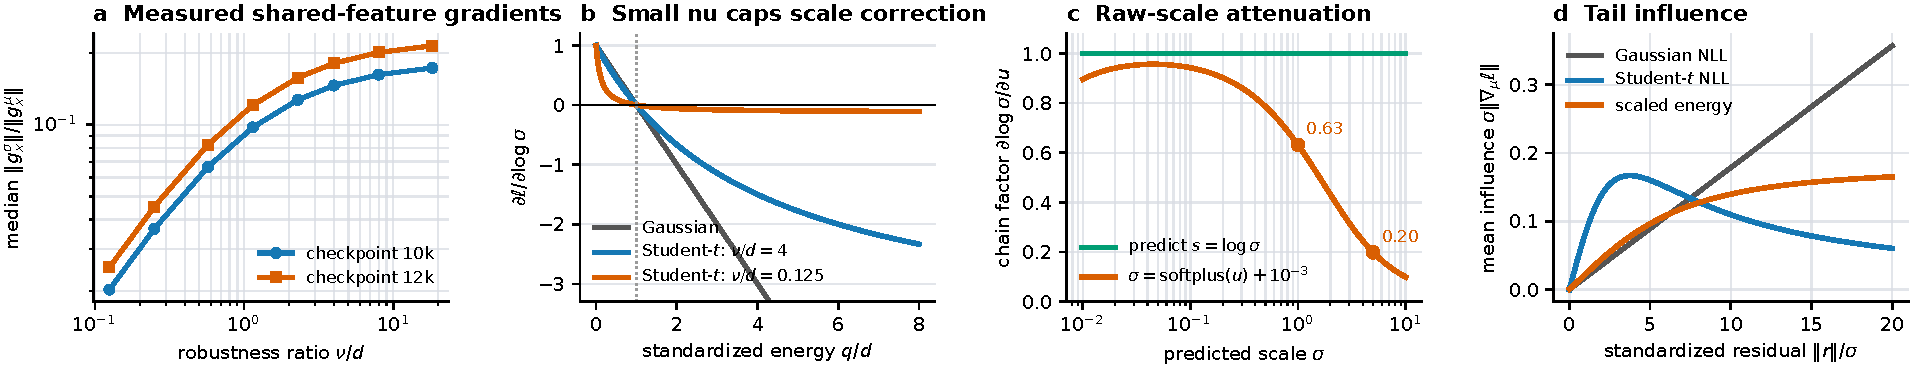
\includegraphics[width=\textwidth]{sigma_gradient_diagnostics.pdf}
\caption{\textbf{两个梯度问题与两种 robust influence。}
(a) 真实 GR00T/Fractal checkpoint 上，减小 $\nu/d$ 后共享特征收到的 scale/mean 梯度比快速下降。
(b) Student-$t$ 的 log-scale score 在 $q/d\gg1$ 时饱和于 $-\nu/d$。
(c) 直接预测 log scale 保持单位链式因子；softplus raw scale 在大 $\sigma$ 时近似按 $1/\sigma$ 衰减。
(d) Gaussian mean influence 随残差无界增长，Student-$t$ redescends 到零；scaled energy influence 有界但不 redescend。只有 (a) 是真实模型测量，(b--d) 是解析或固定随机种子的 Monte Carlo loss 诊断。}
\label{fig:diagnostics}
\end{figure*}

\section{方案 A：detached-mean HG auxiliary 恢复 scale supervision}

用户讨论中的“$\nu$ detach”在实现上应准确写成\textbf{$\mu$ detach}：$\nu$ 本来就是固定常数，没有需要 detach 的计算图。定义
\begin{equation}
 \ell_A
 =\ell_T(\mu,s;\nu)
 +\lambda\,\ell_G(\sg[\mu],s),
 \qquad \lambda\ge0.
 \label{eq:aux-objective}
\end{equation}
stop-gradient 只作用于 auxiliary 的 $\mu$；两个项共享同一个 $\sigma$。

\subsection{为什么梯度方向是对的}

式~\eqref{eq:gradient-identities} 立即给出
\begin{align}
 \nabla_\mu\ell_A
 &=\nabla_\mu\ell_T, \\
 \frac{\partial\ell_A}{\partial s}
 &=\left(\frac{\nu}{\nu+q}+\lambda\right)
 \left(1-\frac{q}{d}\right).
 \label{eq:aux-gradients}
\end{align}
所以 auxiliary 对 direct mean prediction 的梯度严格为零，Student-$t$ 的 robust mean update 完全保留；而 scale 梯度只乘上一个始终为正的系数，其符号仍由 $d-q$ 决定：$q>d$ 时增大 $\sigma$，$q<d$ 时减小 $\sigma$。对单个非零残差，stationary point 仍是 $q=d$，即 $\sigma^2=S/d$。在该点的 log-scale 曲率变为
\begin{equation}
 \left.\frac{\partial^2\ell_A}{\partial s^2}\right|_{q=d}
 =\frac{2\nu}{\nu+d}+2\lambda.
 \label{eq:aux-curvature}
\end{equation}
例如 $d=56,\nu=14,\lambda=1$ 时，从 $0.4$ 提升至 $2.4$，恰好恢复约 $6\times$ 的局部 scale conditioning。

\subsection{它补偿了什么，又没有补偿什么}

\begin{itemize}
 \item \textbf{解决问题一：} HG 项没有 $\nu/(\nu+q)$，因此直接补回小 $\nu$ 丢失的 scale score；detach 保证它不会把 Gaussian 的 unbounded mean gradient 加回去。
 \item \textbf{要解决问题二，仍需 log-scale：} 若继续使用 softplus raw head，式~\eqref{eq:softplus-chain} 仍存在。当前 matched candidate 因此使用 $\sigma=\exp(s)$，而不仅仅是添加 auxiliary。
 \item \textbf{它不是纯 Student-$t$ MLE：} stop-gradient 产生的是一个有意设计的联合更新规则，而不是普通标量目标对 $(\mu,s)$ 的完整梯度。对共享 conditional $\sigma(o)$，HG 与 Student-$t$ 的 population scale optimum 也未必相同。应把它表述为 scale-optimization auxiliary，而不是“仍然精确最大化 Student-$t$ likelihood”。
\end{itemize}

\subsection{已有实验证据}

真实 8-GPU Fractal 首批数据上，$d=56,\nu=14,\lambda=1$：HT-only 的 mean absolute $\log\sigma$ gradient 为 $0.03932$，加入 auxiliary 后为 $0.25671$，提升 $6.53\times$，与式~\eqref{eq:aux-curvature} 的约 $6\times$ 局部预测一致。单元测试同时验证：(i) auxiliary 到 $\mu$ 与 mean-only 参数的梯度严格为零；(ii) 到 $\sigma$ 与共享特征的梯度非零；(iii) combined direct-mean gradient 与 HT-only 完全相同。该证据证明了\emph{梯度机制}，尚未证明最终 closed-loop success 提升。

\section{方案 B：scaled energy proper score}

\subsection{完整定义与严格 propriety}

对任意非退化、具有有限一阶矩的预测分布 $P$，定义
\begin{equation}
 A(P,y)=\E_{X\sim P}\norm{X-y},\qquad
 B(P)=\E_{X,X'\sim P}\norm{X-X'},
\end{equation}
以及待最小化的 scaled energy score
\begin{equation}
 \ell_{SE}(P,y)=\frac{2A(P,y)}{B(P)}+\log B(P).
 \label{eq:scaled-energy-general}
\end{equation}
令真实分布为 $Q$，$C=B(Q)$，$D_E(P,Q)=2\E\norm{X-Y}-B(P)-C$ 为 energy distance，则
\begin{equation}
 \E_Q\ell_{SE}(P,Y)-\E_Q\ell_{SE}(Q,Y)
 =\frac{D_E(P,Q)}{B(P)}+\frac{C}{B(P)}-1+\log\frac{B(P)}{C}\ge0.
 \label{eq:propriety}
\end{equation}
第一项由 energy distance 非负；第二部分在 $B(P)=C$ 时取唯一最小值。故该 score 严格 proper。这里要区分：\emph{score} 可用于广泛的 sampled distributions，但我们的 policy family 若只输出 $(\mu,\sigma)$ 与固定形状 Student-$t$ base distribution，表达能力仍限于这个 location--scale family，并不是“自动表达任意分布”。

\subsection{固定 $\nu$ joint-$t$ 的可训练形式}

令
\begin{equation}
 X=\mu(o)+e^{s(o)}U,qquad U\sim t_\nu(0,I_d),\qquad \nu>1,
\end{equation}
且 $\kappa_{\nu,d}=\E\norm{U-U'}$。因为 $B(P)=e^s\kappa_{\nu,d}$，省略固定常数 $\log\kappa$ 后得到
\begin{equation}
 \ell_{SE}(\mu,s;y)
 =\frac{2}{\kappa_{\nu,d}}\E_U
 \left\| (y-\mu)e^{-s}-U\right\|+s.
 \label{eq:scaled-energy-t}
\end{equation}
它只需在 action vector 空间采样 $U$，不把噪声喂给 policy，也不需要重复网络前向。实验原型固定 $\nu=14,d=56$，用 $K=16$ 个 joint-$t$ samples；一个 chi-square denominator 由整个 56 维向量共享。

\subsection{为什么它能帮助两个 scale 问题}

记 $z=(y-\mu)e^{-s}$、$v(U)=(z-U)/\norm{z-U}$。则
\begin{align}
 \nabla_\mu\ell_{SE}
 &=-\frac{2}{\kappa e^s}\E_U[v(U)],
 &
 \frac{\partial\ell_{SE}}{\partial s}
 &=1-\frac{2}{\kappa}\E_U[z^\top v(U)].
 \label{eq:se-gradients}
\end{align}
它有两个关键性质：
\begin{enumerate}
 \item \textbf{不存在小 $\nu$ 的 scale-score cap。} 式~\eqref{eq:se-gradients} 没有 $\nu/(\nu+q)$ 乘子；当 $\norm{z}$ 很大时，scale gradient 的负向幅值近似随 $\norm{z}$ 线性增长，能够强力纠正被严重低估的尺度。
 \item \textbf{配合 $s=\log\sigma$ 后精确尺度等变。} 同时把 $y-\mu$ 与 $\sigma$ 乘以 $c>0$，$z$ 与 $\partial\ell/\partial s$ 不变；loss 只增加常数 $\log c$。同一组 Monte Carlo base samples 下该性质逐 batch 精确成立。
\end{enumerate}
合成 autograd test 在相同标准化残差下得到：residual RMS/$\sigma=2/1$ 与 $10/5$ 的 $\partial\ell_{SE}/\partial s$ 均为 $-1.352374$。这直接验证了方案 B 对问题二的尺度平衡；analytic constant、mask、joint-$t$ sampling、随机数隔离和 propriety identity 的单元测试均通过。

\subsection{它是否像 Student-$t$ 一样抑制长尾？}

答案是：\textbf{有 bounded mean influence，但不是相同的抑制机制。}
由式~\eqref{eq:se-gradients}，
\begin{equation}
 \norm{\nabla_\mu\ell_{SE}}\le\frac{2}{\kappa\sigma}.
 \label{eq:se-bound}
\end{equation}
因此 outlier 再大，mean gradient 也不会像 Gaussian 那样无界增长。可是当 $\norm{r}/\sigma\rightarrow\infty$ 时，scaled energy 的 mean influence 趋近一个非零常数；Student-$t$ NLL 则按 $1/\norm{r}$ 衰减到零。表~\ref{tab:influence} 总结了差别。

\begin{table}[h]
\centering
\caption{\textbf{三种 score 的尾部 influence。} 令 $R=\norm{r}/\sigma\rightarrow\infty$；忽略与 $R$ 无关的正常数。}
\label{tab:influence}
\small
\begin{tabularx}{0.95\linewidth}{@{}lXXX@{}}
\toprule
Score & Mean influence & Scale correction & 尾部解释 \\
\midrule
Gaussian NLL & $O(R)$，无界 & $O(R^2)$ & outlier 主导 mean 与 scale \\
Student-$t$ NLL & $O(1/R)\to0$ & 饱和于 $-\nu/d$ & redescending；极端样本近似被忽略 \\
Scaled energy & $O(1)$，有界 & $O(R)$ & 限制 mean，但仍让极端样本校正 scale \\
\bottomrule
\end{tabularx}
\end{table}

所以方案 B \emph{相对 Gaussian 确实具有 robust mean fitting}，但不能宣称覆盖或等价于 Student-$t$ 的 redescending robustness。它的 scale gradient 也不是 bounded-robust：真实 contamination 可能推动 $\sigma$ 变大。这既可能是优点（修复 under-estimated conditional scale），也可能是风险（把不可约 outlier 吸收到 scale）；必须由 calibration 与 closed-loop ablation 判断。

\section{两个方案如何选择与验证}

\begin{table}[h]
\centering
\caption{\textbf{两个候选方案的功能边界。}}
\label{tab:solutions}
\small
\begin{tabularx}{\linewidth}{@{}p{0.22\linewidth}XX@{}}
\toprule
 & A: HT + HG($\sg[\mu]$) + log-scale & B: scaled energy + log-scale \\
\midrule
保留 Student-$t$ MLE & Mean gradient 保留；联合更新不再是纯 MLE & 否；改为严格 proper energy score \\
小 $\nu$ scale starvation & HG 项直接补偿 & 没有 $\nu/(\nu+q)$ scale cap \\
绝对尺度平衡 & 需要 exp/log-scale 才完整解决 & exp/log-scale 下精确等变 \\
Mean-tail influence & Student-$t$ redescending & bounded，但不 redescending \\
实现成本 & 无采样；一个 auxiliary & $K$ 个 action-space samples；仍仅一次网络前向 \\
主要风险 & HG scale 项可能吸收 contamination & scale influence 对极端残差无界 \\
\bottomrule
\end{tabularx}
\end{table}

最干净的实验不是直接比较两个新方案，而是做一个能拆开因果因素的 matched ablation：
\begin{enumerate}
 \item native HT + softplus（现有参考）；
 \item native HT + exp/log-scale（只测问题二）；
 \item HT + detached-mean HG + exp（同时补偿问题一、二）；
 \item scaled energy + exp（方案 B）；
 \item scaled energy + softplus（确认方案 B 的收益是否依赖 log-scale）。
\end{enumerate}
所有 arm 必须共享初始 $\sigma_0$、data order、batch、optimizer、训练步数和评价 scenes。训练期同时记录 $\norm{g_x^\sigma}/\norm{g_x^\mu}$、$q/d$、$\sigma$ quantiles、scale-score 正负抵消与 tail gradient mass；最终同时报告 rollout success、held-out NLL/energy score 与 scale calibration。否则“新 score 更好”无法区分是 score、参数化还是初始化造成的。

\section{Claim--evidence map 与当前结论}

\begin{table}[h]
\centering
\caption{\textbf{可安全写入论文的结论与证据状态。}}
\small
\begin{tabularx}{\linewidth}{@{}p{0.34\linewidth}p{0.46\linewidth}p{0.12\linewidth}@{}}
\toprule
Claim & Evidence & Status \\
\midrule
小 $\nu$ 相对抑制 scale path & 精确梯度恒等式；两个真实 checkpoint 的 feature-gradient audit & Supported \\
scale starvation 是性能下降的唯一原因 & 尚无 matched closed-loop causal ablation & Needs evidence \\
softplus raw head 不具绝对尺度等变性 & 精确链式法则；$2/1$ vs. $10/5$ controlled test & Supported \\
detached-mean HG 补偿 scale 且不改 direct mean gradient & 解析式；单元测试；真实首批梯度 $0.03932\to0.25671$ & Supported \\
HG auxiliary 保持纯 Student-$t$ MLE & stop-gradient 与 Gaussian scale target 改变联合估计 & False; do not claim \\
scaled energy 是 strictly proper & energy-distance risk-gap identity & Supported \\
scaled energy 抑制长尾 & mean influence bounded；但不 redescend，scale influence 不 bounded & Qualified \\
任一新方案提高机器人成功率 & matched training/evaluation 尚未完成 & Needs evidence \\
\bottomrule
\end{tabularx}
\end{table}

\paragraph{最终判断。}
目前最强的机制结论不是“理论最优 $\nu$ 应直接拿来训练”，而是：\emph{当 $\nu/d$ 很小时，标准 joint Student-$t$ NLL 同时改变 mean sample weighting 与 scale-head conditioning；现有 raw-scale 参数化又引入第二层尺度不平衡。} 方案 A 是保守修复：保留 Student-$t$ 的 mean robustness，专门补 scale；方案 B 是更统一的 proper-score 修复：用一个 sampled score 同时获得 log-scale 等变性与 bounded mean influence，但放弃 redescending。论文在 closed-loop ablation 完成前，应把二者称为候选优化方案，而不是已经建立的最终算法优势。

\section*{Reviewer-style self-review}
\begin{itemize}
 \item \textbf{Contribution：} 两个失衡是否被明确拆分为 score coupling 与 parameterization coupling？——是。
 \item \textbf{Clarity：} 每个方案是否写清 motivation、definition、gradient 与 limitation？——是。
 \item \textbf{Experimental strength：} 是否已有多个 seed 的 rollout 因果证据？——否，需要 matched ablation。
 \item \textbf{Evaluation completeness：} 是否拆开 auxiliary、score、exp/softplus 与初始化？——已给出必需设计，尚待执行。
 \item \textbf{Soundness：} 是否错误宣称 auxiliary 仍为纯 MLE，或 scaled energy 等价于 Student-$t$ redescending？——没有；两点均明确否定。
\end{itemize}

\section*{Artifacts and references}
\small
\sloppy
\begin{itemize}
 \item Shared-feature gradient audit: \path{analysis/diagnostics/nu_recipe_debug/shared_feature_gradients/}.
 \item $\nu$ switch audit: \path{analysis/diagnostics/nu_gradient_switch/RESULTS.md}.
 \item Auxiliary implementation and tests: \path{scripts/cluster/nu14_gaussian_aux_launch.py}, \path{scripts/cluster/test_nu14_gaussian_aux.py}.
 \item Scaled energy derivation and tests: \path{analysis/diagnostics/nu_recipe_debug/SCALED_ENERGY_DESIGN.md}, \path{scripts/test_scaled_energy_score.py}.
 \item J. E. Bolin and J. Wallin. \emph{Local scale invariance and robustness of proper scoring rules}, 2020.
 \item T. Gneiting and A. E. Raftery. \emph{Strictly proper scoring rules, prediction, and estimation}, JASA, 2007.
 \item K. L. Lange, R. J. A. Little, and J. M. G. Taylor. \emph{Robust statistical modeling using the $t$ distribution}, JASA, 1989.
 \item M. Seitzer et al. \emph{On the pitfalls of heteroscedastic uncertainty estimation with probabilistic neural networks}, ICLR, 2022.
\end{itemize}

\end{document}
